\documentclass[dissertation.tex]{subfiles} 
\begin{document}

\chapter{The Supersymmetric Extension to the Standard Model}
\label{chap:The Supersymmetric Extension to the Standard Model}
%most of this comes from the SUSY primer, but how do I cite it?
%mention MSSM somewhere?

The following introduction to SUSY focuses primarily on the aspects of the formalism that are relevant to phenomenology.  In particular, most of the details of SUSY breaking (about which there is little theoretical consensus) are omitted, except where they are relevant to experiment.

\section{Supermultiplet Representation}
\label{sec:Supermultiplet Representation}

The Standard Model is extended to include supersymmetry by the introduction of a supersymmetry transformation that takes fermionic states to bosonic states and vice versa.  In analogy with the known symmetries of the Standard Model, the SUSY transformation has associated generators that obey defining commutation relations, and a fundamental representation.  All SM particles and their \textit{superpartners} fall into one of two \textit{supermultiplet} representations.  Using the property that

\begin{equation}
n_{F} = n_{B},
\end{equation}
%
where $n_{F}$ is the number of fermionic degrees of freedom per supermultiplet and $n_{B}$ is the number of bosonic degrees of freedom, the two types of supermultiplets are

%increase right margin if committee thinks it looks bad
\begin{enumerate}
  \item \textit{Chiral supermultiplets}: one Weyl fermion (two helicity states $\Rightarrow n_{F} = 2$) and one complex scalar field (with two real components $\Rightarrow n_{B} = 2$)
  \item \textit{Gauge supermultiplets}: One spin-1 vector boson (two helicity states $\Rightarrow n_{B} = 2$) and one Weyl fermion (two helicity states $\Rightarrow n_{F} = 2$)
\end{enumerate}

In the gauge supermultiplet, the vector boson is assumed massless (i.e. before EWSB generates a mass for it).  Since the superpartners to the SM particles have not yet been discovered, they must be significantly heavier than their SM counterparts.  Unbroken SUSY predicts that the SM particles and their superpartners must have exactly the same mass, so ultimately a mechanism for SUSY breaking must be introduced to generate masses for the superpartners (see Sec.~\ref{sec:Soft SUSY Breaking}).  Tables~\ref{tab:chiral_supermultiplets} and~\ref{tab:gauge_supermultiplets} show the chiral and gauge supermultiplets of the supersymmetric Standard Model, respectively.  Note that the scalar partners to the SM fermions are denoted by placing an ``s" in front of their names, while the chiral fermion partners to the SM gauge bosons are denoted by appending ``ino" to their names.

\begin{table}[htbp]
\caption{Chiral supermultiplets of the supersymmetric Standard Model.  Modified from Table 1.1 of \cite{SUSY_primer}.}
\begin{tabular}{|m{3cm}|m{2cm}|m{2cm}|m{2cm}|m{4cm}|}
\hline
Type of \newline supermultiplet & Notation & Spin-0 component & Spin-1/2 component & Representation under $SU(3)_{C} \otimes SU(2)_{L} \otimes U(1)_{Y}$ \\
\hline
\hline
Left-handed quark/squark doublet ($\times$ 3 families) & $Q$ & ($\widetilde{u}_{L}$ $\widetilde{d}_{L}$) & ($u_{L}$ $d_{L}$) & ($\mathbf{3}$, $\mathbf{2}$, $\frac{1}{6}$) \\
\hline
Right-handed up-type quark/squark singlet ($\times$ 3 families) & $\overline{u}$ & $\widetilde{u}_{R}^{*}$ & $u_{R}^{\dag}$ & ($\mathbf{\overline{3}}$, $\mathbf{1}$, $-\frac{2}{3}$) \\
\hline
Right-handed down-type quark/squark singlet ($\times$ 3 families) & $\overline{d}$ & $\widetilde{d}_{R}^{*}$ & $d_{R}^{\dag}$ & ($\mathbf{\overline{3}}$, $\mathbf{1}$, $\frac{1}{3}$) \\
\hline
Left-handed lepton/slepton doublet ($\times$ 3 families) & $L$ & ($\widetilde{\overline{\nu}}_{eL}$ $\widetilde{e}_{L}$) & ($\overline{\nu}_{eL}$ $e_{L}$) & ($\mathbf{1}$, $\mathbf{2}$, $-\frac{1}{2}$) \\
\hline
Right-handed lepton/slepton singlet ($\times$ 3 families) & $\overline{e}$ & $\widetilde{e}_{R}^{*}$ & $e_{R}^{\dag}$ & ($\mathbf{\overline{1}}$, $\mathbf{1}$, 1) \\
\hline
Up-type Higgs/Higgsino doublet & $H_{u}$ & ($H_{u}^{+}$ $H_{u}^{0}$) & ($\widetilde{H}_{u}^{+}$ $\widetilde{H}_{u}^{0}$) & ($\mathbf{1}$, $\mathbf{2}$, $\frac{1}{2}$) \\
\hline
Down-type Higgs/Higgsino doublet & $H_{d}$ & ($H_{d}^{0}$ $H_{d}^{-}$) & ($\widetilde{H}_{d}^{0}$ $\widetilde{H}_{d}^{-}$) & ($\mathbf{1}$, $\mathbf{2}$, $-\frac{1}{2}$) \\
\hline
\end{tabular}
\label{tab:chiral_supermultiplets}
\end{table}

\begin{table}[htbp]
\caption{Gauge supermultiplets of the supersymmetric Standard Model.  Modified from Table 1.2 of \cite{SUSY_primer}.}
\begin{tabular}{|m{5.45cm}|m{2cm}|m{2cm}|m{4cm}|}
\hline
Type of supermultiplet & Spin-1/2 component & Spin-1 component & Representation under $SU(3)_{C} \otimes SU(2)_{L} \otimes U(1)_{Y}$ \\
\hline
\hline
Gluon/gluino & $\widetilde{g}$ & $g$ & ($\mathbf{8}$, $\mathbf{1}$, 0) \\
\hline
W/wino & $\widetilde{W}^{\pm}$ $\widetilde{W}^{0}$ & $W^{\pm}$ $W^{0}$ & ($\mathbf{1}$, $\mathbf{3}$, 0) \\
\hline
B/bino & $\widetilde{B}^{0}$ & $B^{0}$ & ($\mathbf{1}$, $\mathbf{1}$, 0) \\
\hline
\end{tabular}
\label{tab:gauge_supermultiplets}
\end{table}

%%include a section on sparticle masses, cf. Table 7.1 of the SUSY primer?
%The superpartners listed in Tables~\ref{tab:chiral_supermultiplets} and~\ref{tab:gauge_supermultiplets} are not necessarily the mass eigenstates of the theory, because a certain amount of mixing in the gaugino and sfermion sectors is allowed.

%include a section on sparticle decays and production, or an appendix?

%also mention gauge coupling unification

\section{The Unbroken SUSY Lagrangian}
\label{sec:The Unbroken SUSY Lagrangian}

%gauge part --> perform the gauging transformation and break out the full scalar potential

The first piece of the full unbroken SUSY Lagrangian density consists of the kinetic and interacting terms related to the chiral supermultiplets.  As explained in Sec.~\ref{sec:Supermultiplet Representation}, a chiral supermultiplet consists of a Weyl fermion $\psi$ (the ordinary fermion) and a complex scalar $\phi$ (the sfermion).  For a collection of such chiral supermultiplets, the Lagrangian is

\begin{eqnarray}
\label{eq:L_chiral}
\mathcal{L}_{chiral} &=& -\partial^{\mu}\phi^{*i}\partial_{\mu}\phi_{i}\mbox{ }-\mbox{ }V_{chiral}(\phi, \phi^{*})\mbox{ }-\mbox{ }i\psi^{\dag i}\overline{\sigma}^{\mu}\partial_{\mu}\psi_{i}\mbox{ }-\mbox{ }\frac{1}{2}M^{ij}\psi_{i}\psi_{j}\mbox{ }\nonumber \\
&&-\mbox{ }\frac{1}{2}M_{ij}^{*}\psi^{\dag i}\psi^{\dag j}\mbox{ }-\mbox{ }\frac{1}{2}y^{ijk}\phi_{i}\psi_{j}\psi_{k}\mbox{ }-\mbox{ }\frac{1}{2}y_{ijk}^{*}\phi^{*i}\psi^{\dag j}\psi^{\dag k}
\end{eqnarray}
%put more horizontal space here
where $i$ runs over all supermultiplets in Table~\ref{chiral_supermultiplets}, $\overline{\sigma}^{\mu}$ are -1 $\times$ the Pauli matrices (except for $\sigma^{0}$ = $\overline{\sigma}^{0}$), $M^{ij}$ is a mass matrix for the fermions, $y^{ijk}$ are the Yukawa couplings between one scalar and two spinor fields, and $V_{chiral}(\phi, \phi^{*}$ is the scalar potential

\begin{eqnarray}
\label{eq:V_chiral}
V_{chiral}(\phi, \phi^{*}) &=& M_{ik}^{*}M^{kj}\phi^{*i}\phi_{j}\mbox{ }+\mbox{ }\frac{1}{2}M^{in}y_{jkn}^{*}\phi_{i}\phi^{*j}\phi^{*k}\mbox{ }\nonumber \\
&&+\mbox{ }\frac{1}{2}M_{in}^{*}y^{jkn}\phi^{*i}\phi_{j}\phi_{k}\mbox{ }+\mbox{ }\frac{1}{4}y^{ijn}y_{kln}^{*}\phi_{i}\phi_{j}\phi^{*k}\phi^{*l}.
\end{eqnarray}
%
The Lagrangian can also be written as the kinetic terms plus derivatives of the \textit{superpotential} $W$:

\begin{eqnarray}
\label{eq:L_chiral_W}
\mathcal{L}_{chiral} &=& -\partial^{\mu}\phi^{*i}\partial_{\mu}\phi_{i}\mbox{ }-\mbox{ }i\psi^{\dag i}\overline{\sigma}^{\mu}\partial_{\mu}\psi_{i}\mbox{ }\nonumber \\
&&-\mbox{ }\frac{1}{2}(\frac{\delta^{2}W}{\delta\phi^{i}\delta\phi^{j}}\psi_{i}\psi_{j} + \frac{\delta^{2}W^{*}}{\delta\phi_{i}\delta\phi_{j}}\psi^{\dag i}\psi^{\dag j})\mbox{ }-\mbox{ }\frac{\delta W}{\delta\phi^{i}}\frac{\delta W^{*}}{\delta\phi_{i}}
\end{eqnarray}
%
where

\begin{eqnarray}
\label{eq:W}
W &=& M^{ij}\phi_{i}\phi_{j}\mbox{ }+\mbox{ }\frac{1}{6}y^{ijk}\phi_{i}\phi_{j}\phi_{k}.
\end{eqnarray}

%define the sigmabar above
The second part of the Lagrangian involves the gauge supermultiplets.  In terms of the spin-1 ordinary gauge boson $A_{\mu}^{a}$ and the spin-1/2 Weyl spinor gaugino $\lambda^{a}$ of the gauge supermultiplet, where $a$ runs over the number of generators for the SM subgroup (i.e. 1-8 for $SU(3)_{C}$, 1-3 for $SU(2)_{L}$, and 1 for $U(1)_{Y}$), this part of the Lagrangian is

\begin{eqnarray}
\label{eq:L_gauge}
\mathcal{L}_{gauge} &=& -\frac{1}{4}F_{\mu\nu}^{a}F^{\mu\nu a}\mbox{ }-\mbox{ }i\lambda^{\dag a}\overline{\sigma}^{\mu}D_{\mu}\lambda^{a}\mbox{ }+\mbox{ }\frac{1}{2}D^{a}D^{a}
\end{eqnarray}
%
where 

\begin{eqnarray}
\label{eq:F}
F_{\mu\nu}^{a} &=& \partial_{\mu}A_{\nu}^{a}\mbox{ }-\mbox{ }\partial_{\nu}A_{\mu}^{a}\mbox{ }+\mbox{ }gf^{abc}A_{\mu}^{b}A_{\nu}^{c}
\end{eqnarray}
%
($g$ is the coupling constant and $f^{abc}$ are the structure constants for the particular SM gauge group), 

\begin{eqnarray}
\label{eq:gaugino_covariant_derivative}
D_{\mu}\lambda^{a} &=& \partial_{\mu}\lambda^{a}\mbox{ }+\mbox{ }gf^{abc}A_{\mu}^{b}\lambda^{c}, 
\end{eqnarray}
%
and $D^{a}$ is an auxiliary field that does not propagate (in the literature, it is used as a bookkeeping tool and can be removed via its algebraic equation of motion).

To build a fully supersymmetric and gauge-invariant Lagrangian, the ordinary derivatives in $\mathcal{L}_{chiral}$ (Eq.~\ref{eq:L_chiral}) must be replaced by covariant derivatives

\section{Soft SUSY Breaking}
\label{sec:Soft SUSY Breaking}

%unbroken SUSY Lagrangian
%addition of soft SUSY-breaking terms and motivation for soft terms
%how to avoid flavor violation
%sparticle masses and RG evolution
%unification of couplings at high scale

\section{Dark Matter and the WIMP Miracle}
\section{Gauge-Mediated SUSY Breaking}
\label{sec:Gauge-Mediated SUSY Breaking}
%minimal
%general -- also describe bino-like vs. wino-like in terms of M1 and M2, say it will be important later
%gravitino LSP because it is so light because of low-scale SUSY breaking
%phenomenological differences
%neutralino lifetime and mass equations
\section{Experimental Status of SUSY}

Collider searches for evidence of supersymmetry began in earnest in the 1980s \cite{SUSY_history} and continue to this day.  Most recently, the LHC and Tevatron\footnote{Located on the Fermilab site in Batavia, Illinois, the Tevatron was a proton-antiproton collider operating at 1.96 TeV center-of-mass energy.  The Tevatron ran from 1987 to 2011 \cite{Tevatron_lifetime}.} experiments have set the strictest limits on a variety of SUSY breaking scenarios, including GMSB and mSUGRA (discussed below).

Figure~\ref{fig:CMS_SUSY_2011Limits_tanb10} shows the current limits set by the CMS experiment on the mSUGRA model (with tan $\beta$ = 10) in the $m_{0}$-$m_{1/2}$ plane.  (Note that although the plot is truncated at $m_{0}$ = 1000 GeV/$\mbox{c}^{2}$, some searches are sensitive out to $m_{0} \sim$ 2000 GeV/$\mbox{c}^{2}$.)  Although the LHC has pushed $m_{0}$ above $\sim$1 TeV/$\mbox{c}^{2}$ for $m_{1/2}$ up to $\sim$400 GeV/$\mbox{c}^{2}$, casting some doubt onto the theory's prospects for solving the hierarchy problem, there is still a sizable chunk of mSUGRA parameter space that is not ruled out by collider experiments.  Furthermore, parts of the CMS unexplored regions overlap with areas allowed by astrophysics experiments \cite{CMSSM_fits}.

\begin{figure}
	\centering
	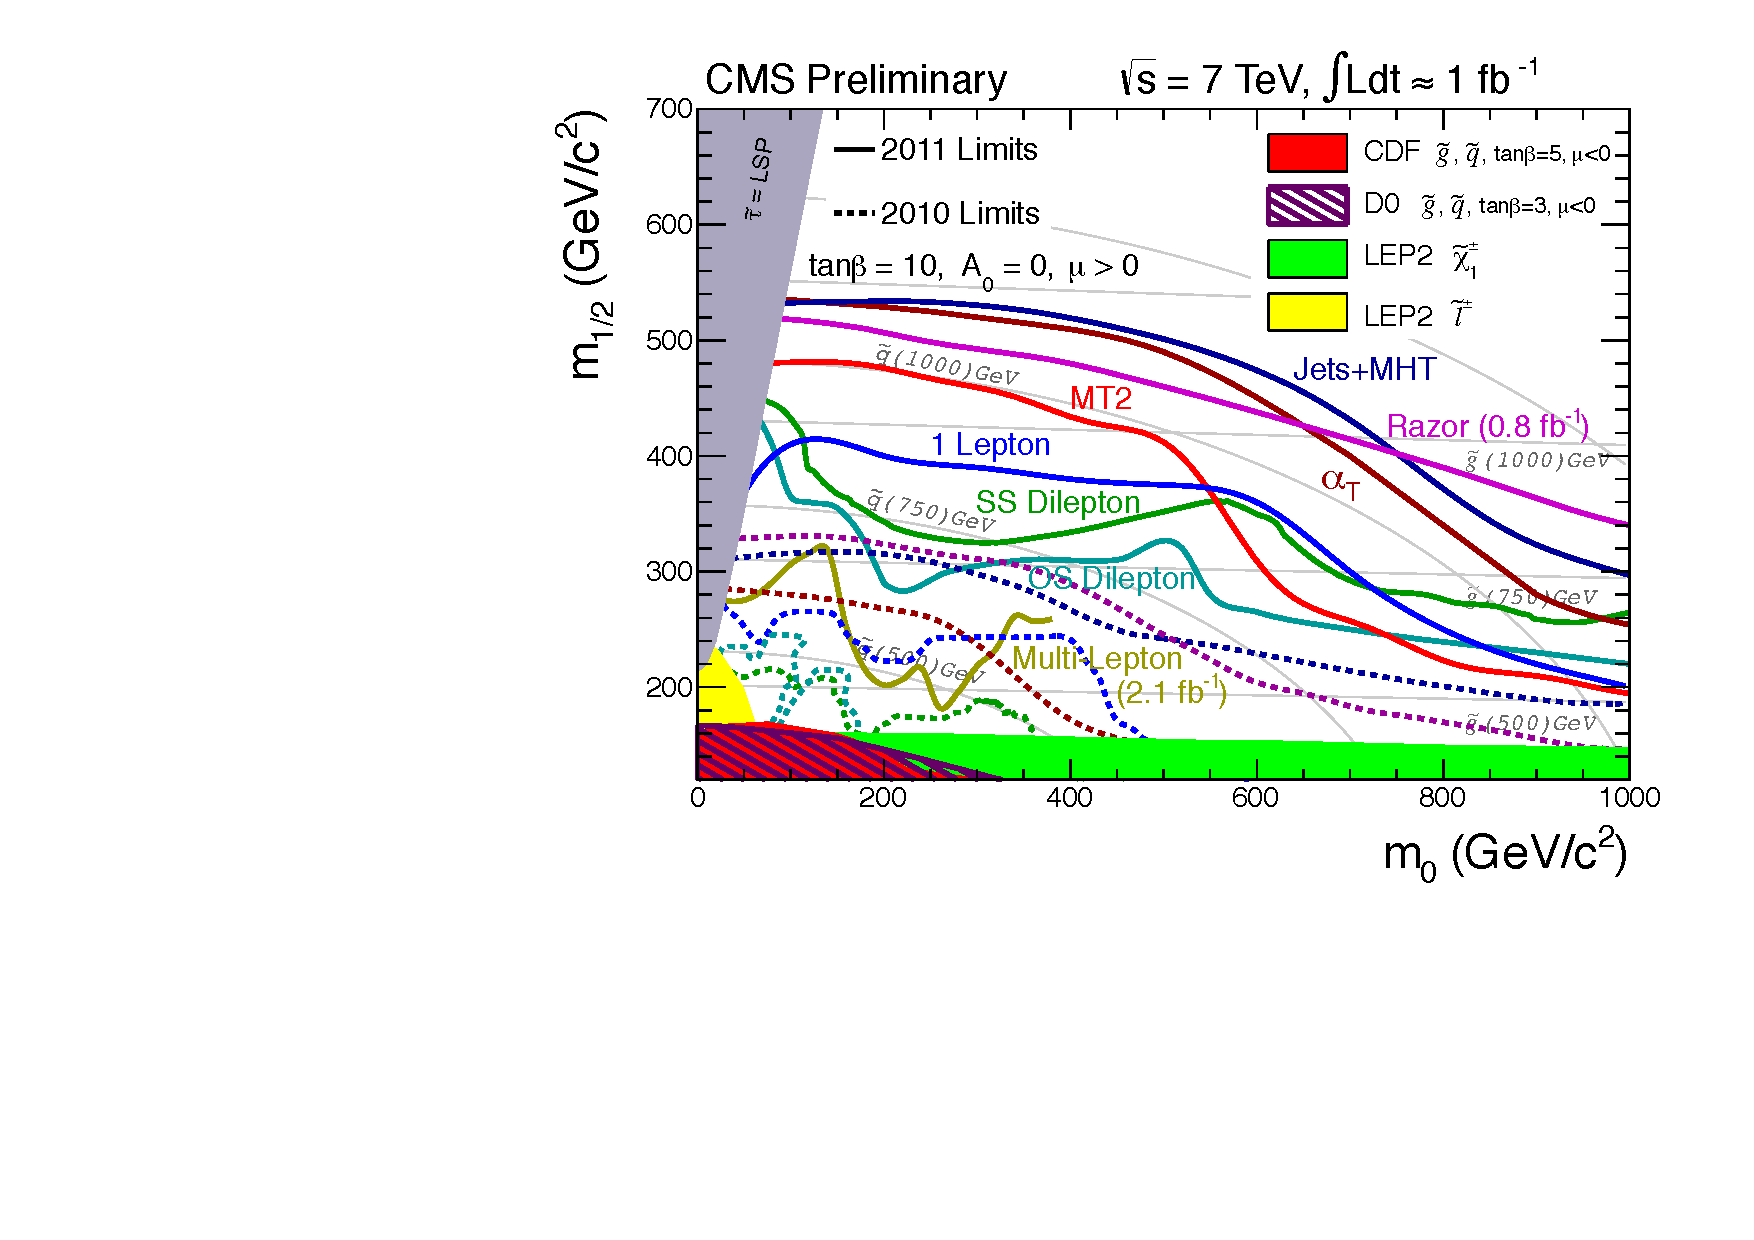
\includegraphics[scale=0.6]{CMS_SUSY_2011Limits_tanb10}
	\caption{CMS limits on mSUGRA with tan $\beta$ = 10.  The limits set by individual searches are shown as separate colored lines.  Solid lines refer to 2011 searches (i.e. using an integrated luminosity of $\sim$1 $\mbox{fb}^{-1}$), while dashed lines refer to 2010 searches ($\sim$36 $\mbox{pb}^{-1}$).  Reprinted from \cite{CMS_mSUGRA}.}
	\label{fig:CMS_SUSY_2011Limits_tanb10}
\end{figure}

%check this whole paragraph and figures from ATLAS!
Figure~\ref{fig:ATLAS_SPS8_limit} shows the most up-to-date limit (using 1 $\mbox{fb}^{-1}$ of integrated luminosity collected by the ATLAS experiment \cite{ATLAS} at the LHC) on the Snowmass Points and Slopes (SPS) model of minimal GMSB (mGMSB), dubbed SPS8 \cite{SPS}.  SPS8 represents the simplest class of GMSB models described in Sec.~\ref{sec:Gauge-Mediated SUSY Breaking}.  The best limits on a variety of general gauge mediation (GGM) models, from the same ATLAS study, are shown in Figure~\ref{fig:ATLAS_GGM_limit}.  In these models, no assumptions are made about the specific parameters common to many gauge mediation models (e.g. the number of messengers or the relationship between the messenger mass and the SUSY breaking scale).  Instead, it is only assumed that the lightest neutralino is light enough to be produced on-shell at the LHC (by setting $\mbox{M}_{1}$ and $\mbox{M}_{2}$ appropriately, see Sec.~\ref{SUSY Lagrangian and Particle Content, SUSY Breaking}) and that it decays to a gravitino, that the gravitino is extremely relativistic (mass of order eV-keV), and that the gravitino is stable.  The one-dimensional scan over SUSY breaking scales in the SPS8 model (in which the full sparticle spectrum is specified by the model parameters) is replaced by a two-dimensional scan over gluino and lightest neutralino mass in the GGM models (in which all sparticles except the gluino, first- and second-generation squarks, and neutralinos are forced to be at $\sim$1.5 TeV/$\mbox{c}^{2}$, effectively decoupling them from the dynamics that can be probed with 1 $\mbox{fb}^{-1}$ at a 7 TeV/c pp collider).
%maybe repeat some of this in the earlier section about the advantages of simplified models (can make a more logical, clear mapping between search strategy and model sensitivity, can be less model-dependent)

\begin{figure}
	\centering
	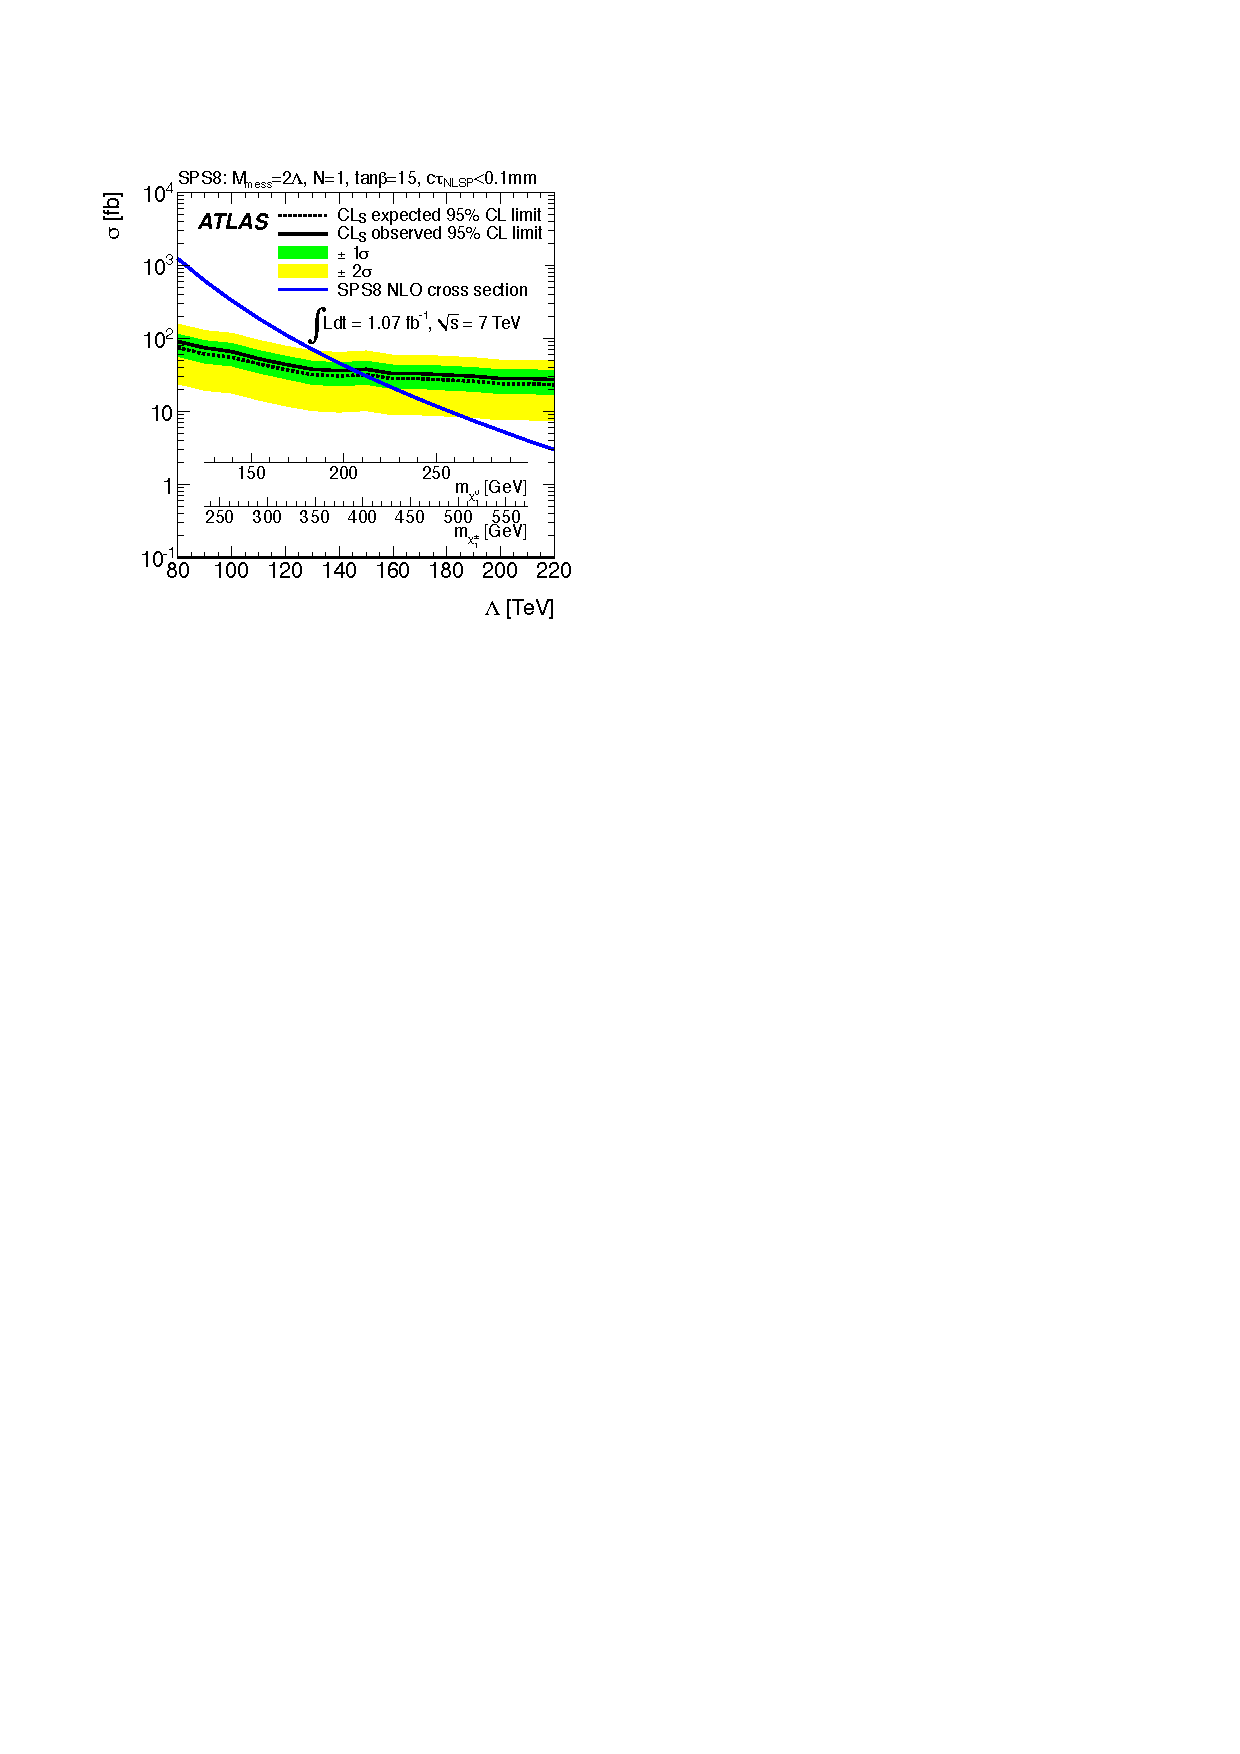
\includegraphics[scale=0.9]{ATLAS_SPS8_limit}
	\caption{ATLAS cross section upper limit on the SPS8 \cite{SPS} model of mGMSB as a function of SUSY breaking scale $\Lambda$, lightest neutralino mass $\mbox{m}_{\NLSP}$, or lightest chargino mass $\mbox{m}_{\widetilde{\chi}_{1}^{\pm}}$.  Values of $\Lambda$, $\mbox{m}_{\NLSP}$, or $\mbox{m}_{\widetilde{\chi}_{1}^{\pm}}$ below the intersection point between the blue (predicted SPS8 cross section) and black (observed cross section upper limit) curves are excluded.  The model parameters listed above the plot are defined in Sec.~\ref{sec:Gauge-Mediated SUSY Breaking}.  Reprinted from \cite{ATLAS_GMSB_1fb-1}.}
	\label{fig:ATLAS_SPS8_limit}
\end{figure}

\begin{figure}
	\centering
	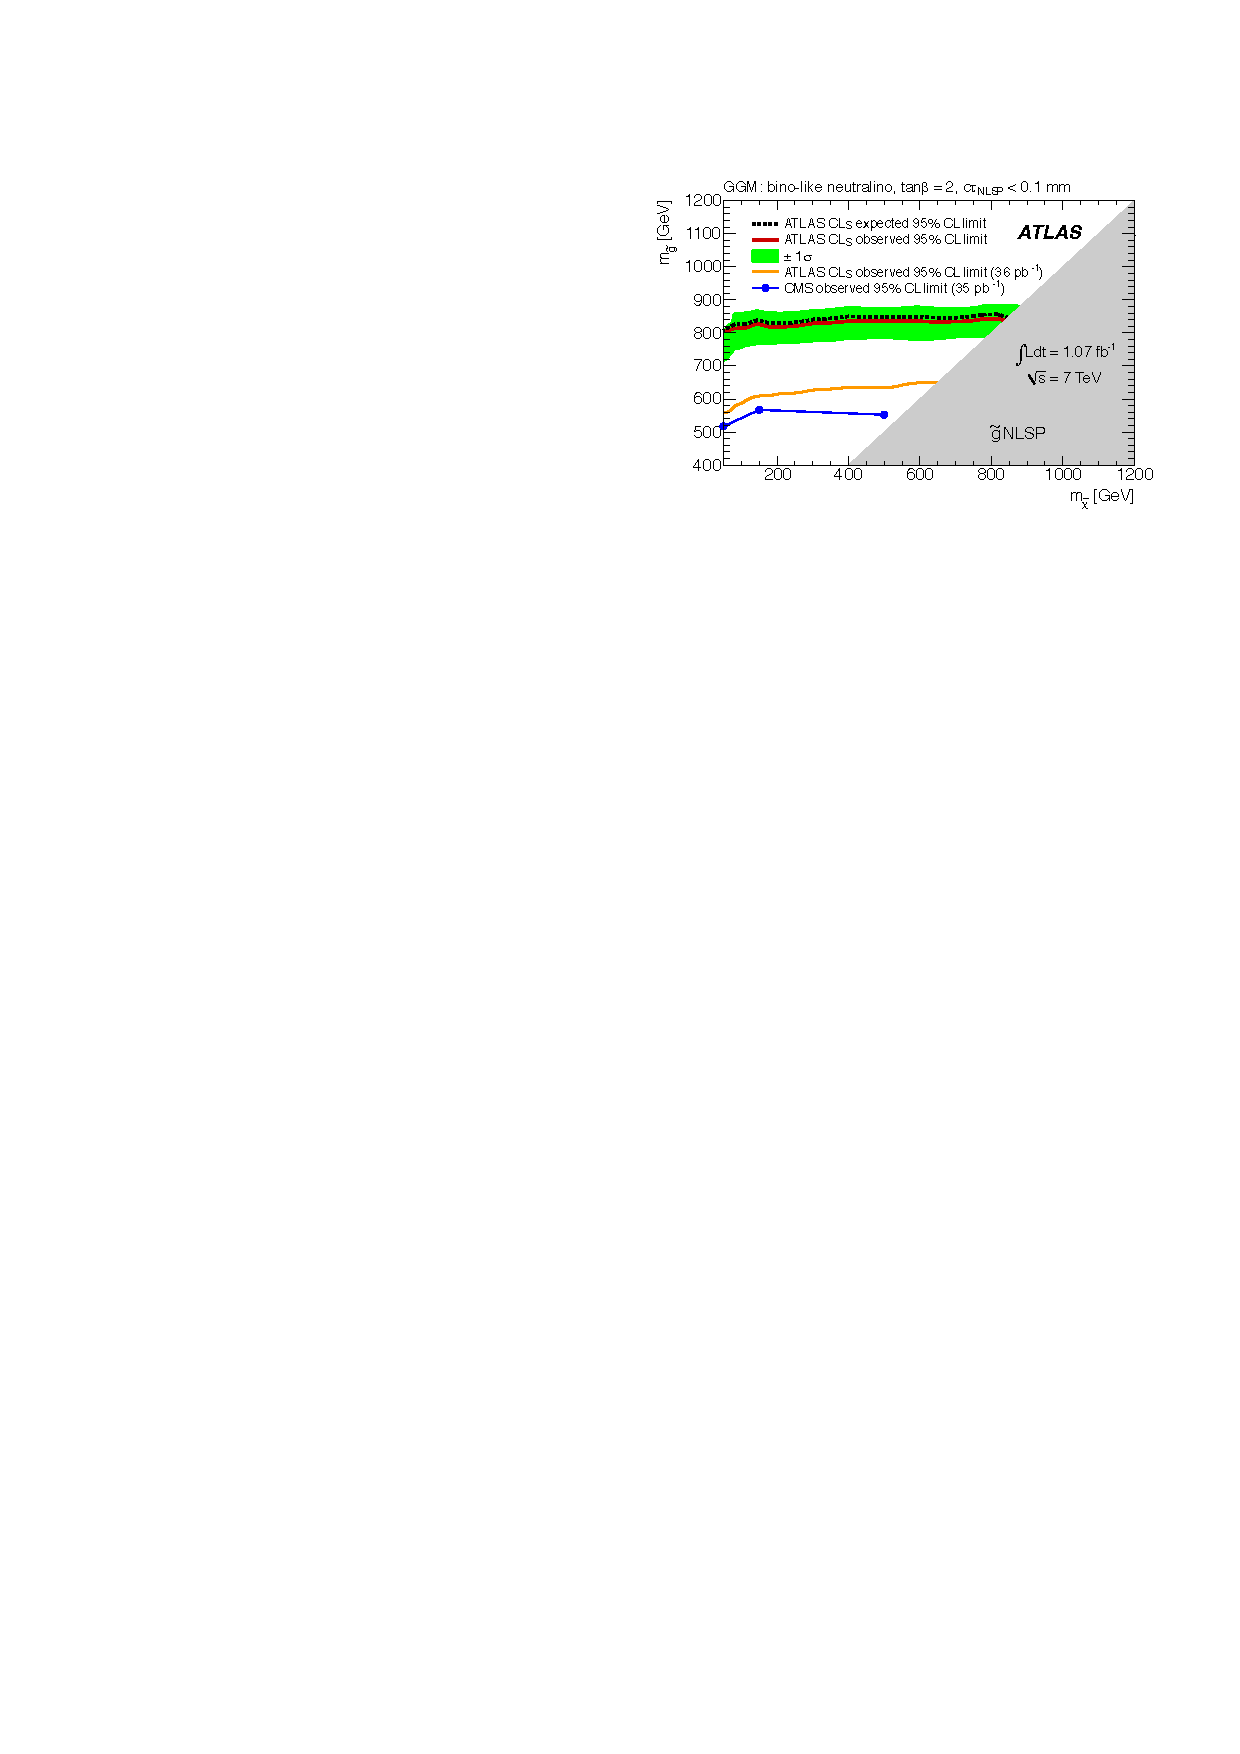
\includegraphics[scale=0.9]{ATLAS_GGM_limit}
	\caption{ATLAS exclusion contour in the $\mbox{m}_{\widetilde{\mbox{g}}}$-$\mbox{m}_{\NLSP}$ plane.  Values of $\mbox{m}_{\widetilde{\mbox{g}}}$-$\mbox{m}_{\NLSP}$ below the red curve are excluded.  The gray region is theoretically excluded in the GGM models considered.  ``Bino-like neutralino" means that $\mbox{M}_{2}$ = 1.5 TeV/$\mbox{c}^{2}$.  Reprinted from \cite{ATLAS_GMSB_1fb-1}.}
	\label{fig:ATLAS_GGM_limit}
\end{figure}

In general, the lifetime of the lightest neutralino in GMSB models can take on any value between hundreds of nanometers to a few kilometers depending on the mass of the lightest neutralino and the SUSY breaking scale \cite{SUSY_primer}.  The search published in \cite{ATLAS_GMSB_1fb-1} (from which Figs.~\ref{fig:ATLAS_SPS8_limit} and~\ref{fig:ATLAS_GGM_limit} are culled) considers only \textit{prompt} neutralino variants, i.e. with neutralino lifetime short enough that the distance traveled by the neutralino before decay cannot be resolved by the detector.  The most recent limits on non-prompt SPS8-style neutralino models were set by the Collider Detector at Fermilab (CDF) collaboration with 570 $\mbox{pb}^{-1}$, and are shown in Figure~\ref{fig:CDF_lifetime_vs_mass} \cite{CDF_2010_GMSB_paper}.

\begin{figure}
	\centering
	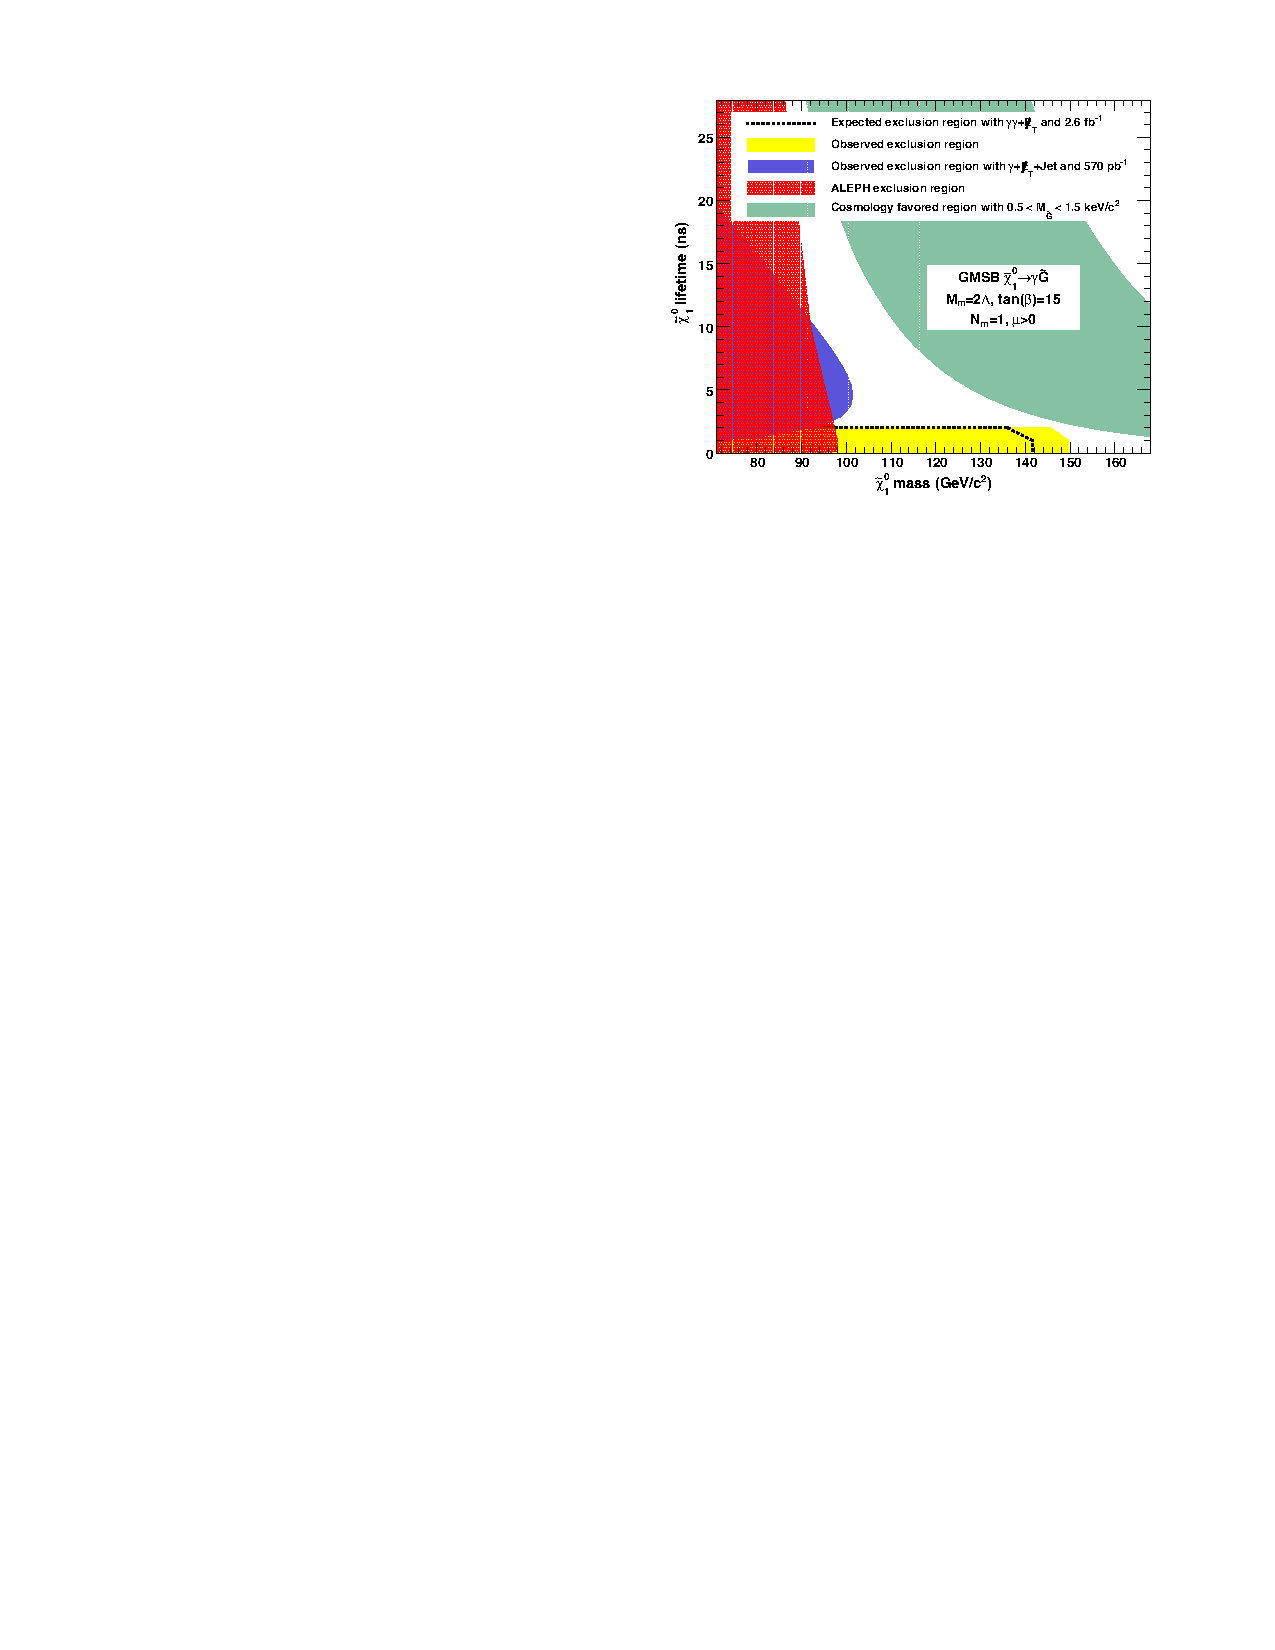
\includegraphics[scale=1.0]{CDF_lifetime_vs_mass}
	\caption{CDF exclusion contour in the $\tau_{\NLSP}$-$\mbox{m}_{\NLSP}$ plane, where $\tau_{\NLSP}$ is the lifetime of the neutralino.  Reprinted from \cite{CDF_2010_GMSB_paper}.}
	\label{fig:CDF_lifetime_vs_mass}
\end{figure}

Finally, if the gravitino is to make up some or all of the dark matter, constraints on the form of gauge mediation must come from cosmological considerations and astronomical observations.  The gravitino in gauge mediation models is usually very light ($\mathcal{O}$(eV-MeV)) because it is proportional to the SUSY breaking scale divided by the Planck mass, and in GMSB the breaking scale is typically only of order a few hundred TeV (\cite{SUSY_primer} and Sec.~\ref{sec:SUSY Lagrangian and Particle Content, SUSY Breaking}).  A light, highly relativistic dark matter particle might have been produced, for instance, in the early, radiation-dominated period of the universe \cite{Lyman_alpha_DM_limits}.  This \textit{warm dark matter} (WDM) may be responsible for all of the dark matter needed to account for galactic structure, or it may share the duties with \textit{cold dark matter} (CDM, the classic WIMPs of Sec.~\ref{sec:SUSY Lagrangian and Particle Content, SUSY Breaking}).  In any viable model, the predicted relic density of the dark matter species must match the observed value of $\Omega \mbox{h}^{2} \sim$ 0.1 \cite{WMAP}.  For many GMSB models, this measurement constrains the gravitino mass to the keV range \cite{long_lived_neutralinos_at_the_Tevatron}.  This constraint, however, does not translate into a very strong bound on the lifetime of the lightest neutralino.  Using the following equation (taken from \cite{long_lived_neutralinos_at_the_Tevatron}):

\begin{equation}
\tau_{\NLSP} \sim 130(\frac{100 \mbox{GeV}}{\mbox{m}_{\NLSP}})^{5}(\frac{\sqrt{\mbox{F}}}{100 \mbox{TeV}})^{4}\mbox{ }\mu \mbox{m}
\end{equation}
%
where $\sqrt{\mbox{F}}$ is approximately the SUSY breaking scale, and applying the gravitino mass constraint $\sqrt{\mbox{F}}$ $\lesssim$ 3000 TeV (cf. Eq. X with $\mbox{m}_{\widetilde{G}} \sim$ keV) and $\mbox{m}_{\NLSP}$ = 100 GeV, the upper bound on the neutralino lifetime is 100 meters.  For $\sqrt{\mbox{F}} \sim$ 100 TeV, the neutralino lifetime is detectable on collider time scales.

Recently, a lower bound on the WDM particle mass in either pure warm or mixed warm and cold dark matter scenarios was set using observations of the Lyman-$\alpha$ forest.  For pure WDM, $\mbox{m}_{\mbox{WDM}} >$ 8 keV, while for some mixed WDM-CDM scenarios, $\mbox{m}_{\mbox{WDM}} >$ 1.1-1.5 keV \cite{Lyman_alpha_DM_limits, cosmo_constraints_on_GMSB}.  These bounds and others have motivated the development of more complicated gauge mediation models \cite{cosmo_constraints_on_GMSB}.  However, rather than focus on a specific GMSB model, of which there are many, the search detailed here is interpreted in a minimally model dependent way.  With this approach, the results can be applied to many competing models.  The remainder of this thesis is devoted to the experimental details of the search, analysis strategy, and presentation of the results.

\end{document}